The goal of the project is to analyze the IMDb Dataset, which contains data about movies, TV shows, and other forms of visual entertainment, along with their ratings.
Each record includes key information about the title, as well as insights into critical aspects such as awards and reviews, as well as statistical ratings and other metadata. The dataset is updated as of September 1, 2024.

\subsection{Data Semantics and First Global Exploration of the Dataset}
\label{data_semantics}
The IMDb Dataset contains 16431 records and 23 attributes, of which 10 are categorical and 13 numeric. They are listed in Tables \ref{tab:original_vars_num} and \ref{tab:original_vars_cat}.
Among the \textbf{numerical attributes}, most of them are discrete and ratio-scaled, as they represent counts, with \textit{startYear} and \textit{endYear} being interval values.
Only \textit{runtimeMinutes} can be classified as a continuous attribute, as it represents a time duration, even though it only assumes integer values in the dataset.
Among the \textbf{categorical attributes}, \textit{canHaveEpisodes}, \textit{isRatable} and \textit{isAdult} are \textbf{binary}, \textit{rating }, \textit{worstRating} and \textit{bestRating} are \textbf{ordinal}, while the rest are all \textbf{nominal}.

Looking at the records' data types, we can observe some syntactic inaccuracies: \textit{isAdult }should be converted from integer to boolean, whereas \textit{rating} assumes ten categorical values of the form  \textit{'(0, 1]', '(1, 2]', ..., '(9, 10]'}. We can assume they represent the binning of a continuous rating, therefore we map them into an integer space [1,10] to ease later analysis. Just by looking at the head of the dataframe, we can also tell that \textit{countryOfOrigin} and \textit{genres} contain collections of categorical values; therefore, we transform them into lists to allow for easier handling. Some discrete numerical attributes (\textit{endYear}, \textit{awardWins}) are stored as float rather than boolean because \texttt{int64} does not support NaN values; however, we do not deem it necessary to convert them.

\begin{table*}[h]
    \centering
    \renewcommand{\arraystretch}{1.2}
    \scriptsize
    \begin{tabular}{|p{3cm}|p{5cm}|p{1.5cm}|p{1.5cm}|}
    \hline
    \textbf{Feature} & \textbf{Description} & \textbf{Type} & \textbf{Pandas dtype} \\ \hline
    runtimeMinutes & Primary runtime of the title, in minutes. & Continuous. Ratio-scaled. & float64 \\ \hline
    startYear & Represents the release year of a title. In the case of TV Series, it is the series' start year. & Discrete. Interval. & int64 \\ \hline
    endYear & TV Series end year. & Discrete. Interval. & float64 \\ \hline
    ratingCount & The total number of user ratings submitted for the title. & Discrete. Ratio-scaled. & int64 \\ \hline
    numVotes & Number of votes the title has received. & Discrete. Ratio-scaled. & int64 \\ \hline
    numRegions & The regions number for this version of the title. & Discrete. Ratio-scaled. & int64 \\ \hline
    totalImages & Total Number of Images for the title within the IMDb title page. & Discrete. Ratio-scaled. & int64 \\ \hline
    totalVideos & Total Number of Videos for the title within the IMDb title page. & Discrete. Ratio-scaled. & int64 \\ \hline
    totalCredits & Total Number of Credits for the title. & Discrete. Ratio-scaled. & int64 \\ \hline
    criticsReviewTotal & Total Number of Critic Reviews. & Discrete. Ratio-scaled. & int64 \\ \hline
    awardWins & Number of awards the title won. & Discrete. Ratio-scaled. & float64 \\ \hline
    awardNominationExclWins & Number of award nominations excluding wins. & Discrete. Ratio-scaled. & int64 \\ \hline
    userReviewsTotal & Total Number of Users Reviews. & Discrete. Ratio-scaled. & int64 \\ \hline
    \end{tabular}
    \caption{Numeric attributes.}
    \label{tab:original_vars_num}
\end{table*}

\begin{table*}[h]
    \centering
    \renewcommand{\arraystretch}{1.2}
    \scriptsize
    \begin{tabular}{|p{2cm}|p{4.5cm}|p{3cm}|p{1.5cm}|}
        \hline
        \textbf{Feature} & \textbf{Description} & \textbf{Type} & \textbf{Pandas dtype} \\ \hline
        originalTitle & Original title, in the original language. & Categorical; mostly unique classes (i.e., names). & object \\ \hline
        titleType & The type/format of the title (e.g., movie, short, episode, video, etc.). & Categorical, 10 classes. & object \\ \hline
        countryOfOrigin & The country where the title was primarily produced. Some titles can belong to more than one class. & Categorical, 153 classes. A record can belong to more than one class. & object \\ \hline
        genres & The genre(s) associated with the title (e.g., drama, comedy, action). Some titles can belong to more than one class. & Categorical, 29 classes. A record can belong to more than one class. & object \\ \hline
        canHaveEpisodes & Whether or not the title can have episodes. & Asymmetric binary. & bool \\ \hline
        isRatable & Whether or not the title can be rated by users. & Asymmetric binary. & bool \\ \hline
        isAdult & Whether or not the title is for adults. & Asymmetric binary. & int64 \\ \hline
        rating & IMDB title rating class. & Ordinal, 10 values. & object \\ \hline
        worstRating & Worst title rating. & Ordinal, supposedly [1,10]. & int64 \\ \hline
        bestRating & Best title rating. & Ordinal, supposedly [1,10]. & int64 \\ \hline
    \end{tabular}
    \caption{Categorical, ordinal, and binary attributes.}
    \label{tab:original_vars_cat}
\end{table*}

A first global analysis of the dataframe's summary and descriptive statistics already gives us valuable insight into which variables have missing values\footnote{As the missing values were recorded inconsistently in the dataset, we used the \texttt{read\_csv} function, passing a list of strings to recognize as missing values to the parameter \texttt{na\_values}.}, as reported in Table \ref{tab:feats_nan}, and into which features are uninformative: \textit{bestRating}, \textit{worstRating}, and \textit{isRatable} can be safely dropped, as they only assume one value for all records (10, 1, and 1, respectively). We can also see that \textit{numVotes} and \textit{ratingCount} share very similar, when not identical, statistics. The scatterplot in Figure \ref{fig:scatterplot_numVotes_ratingCount} proves their correlation close to 1, which leads us to drop \textit{ratingCount} and only keep \textit{numVotes}.

\begin{table}[h]
    \centering
    \caption{Features with missing values.}
    \begin{tabular}{|l|r|}
        \hline
        \textbf{Feature} & \textbf{Non-Null Records} \\
        \hline
        endYear & 814 \\
        runtimeMinutes & 11579 \\
        awardWins & 13813 \\
        genres & 16049 \\
        \hline
    \end{tabular}
    \label{tab:feats_nan}
\end{table}

\begin{figure}
    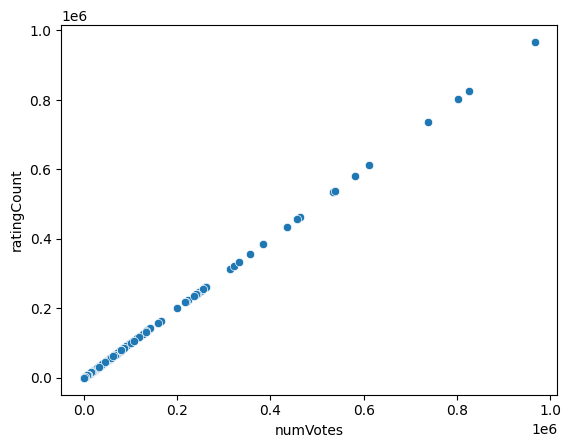
\includegraphics[width=\columnwidth]{../results/images/scatter_numVotes_ratingCount.png}
    \caption{Scatterplot ratingCount\textasciitilde numVotes.}
    \label{fig:scatterplot_numVotes_ratingCount}
\end{figure}

\subsection{Distribution of categorical variables and statistics}
In an effort to analyze the univariate distribution of categorical variables, we produced barplots for \textit{titleType} (Figure \ref{fig:barplot_titleType.png}), \textit{countryOfOrigin} (Figure \ref{fig:barplot_countryOfOrigin.png}), and \textit{genres} (Figure \ref{fig:barplot_genres.png}). All distributions are imbalanced, being dominated by few very common classes: \textit{movie} and \textit{tvepisode}, the \textit{US}, \textit{drama} and \textit{comedy}, respectively. A barplot for \textit{rating}\footnote{In this data exploration phase, we analyzed this ordinal variable both from a categorical and a numeric point of view, as to maximize insights.}, in Figure \ref{fig:barplot_rating.png}, shows a left-skewed distribution, with the mode being the [7,8) category.

\begin{figure}
    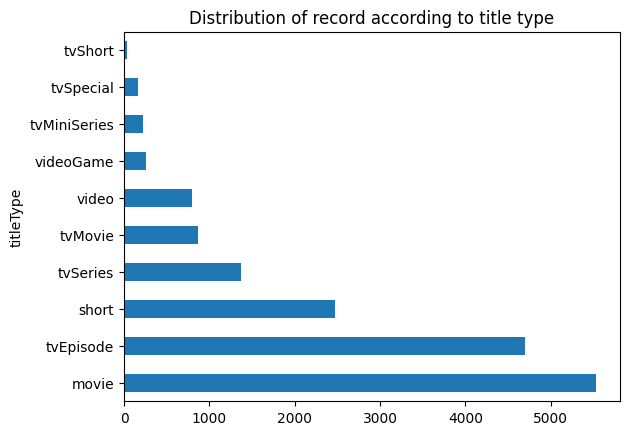
\includegraphics[width=\columnwidth]{../results/images/barplot_titleType.png}
    \caption{Barplot for \textit{titleType}.}
    \label{fig:barplot_titleType.png}
\end{figure}

\begin{figure}
    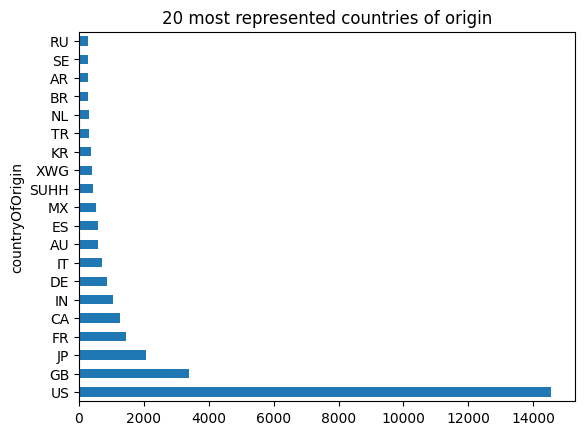
\includegraphics[width=\columnwidth]{../results/images/barplot_countryOfOrigin.png}
    \caption{Barplot for \textit{countryOfOrigin} (top 20).}
    \label{fig:barplot_countryOfOrigin.png}
\end{figure}

\begin{figure}
    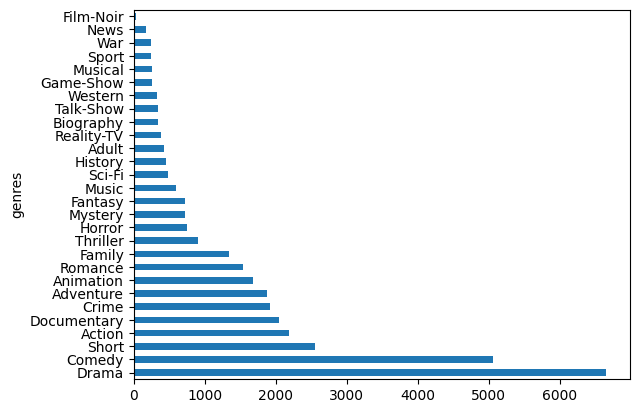
\includegraphics[width=\columnwidth]{../results/images/barplot_genres.png}
    \caption{Barplot for \textit{genres}.}
    \label{fig:barplot_genres.png}
\end{figure}

\begin{figure}
    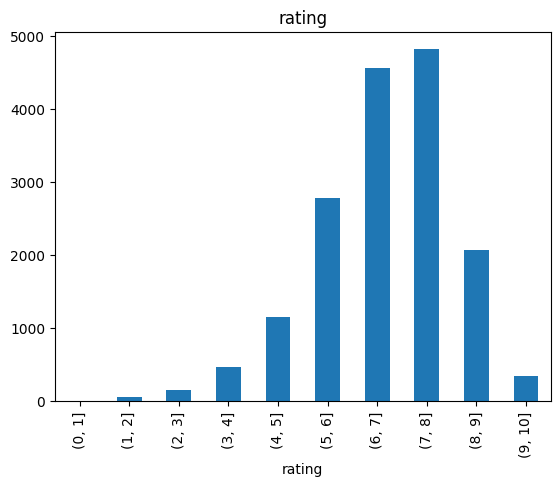
\includegraphics[width=\columnwidth]{../results/images/barplot_rating.png}
    \caption{Barplot for \textit{rating}.}
    \label{fig:barplot_rating.png}
\end{figure}

By looking at the categories for the different variables, we question the informativeness of \textit{canHaveEpisodes} and \textit{isAdult}. The first assumes positive values only for the title types \textit{tvSeries} and \textit{tvMiniSeries}:  we keep it, as an explicit feature of serialized content. \textit{isAdult} proves to be redundant as its information is conveyed by the \textit{adult} category in \textit{genres}, therefore we drop it.

\subsection{Distribution of numeric variables and statistics; transformation of variables}
\label{numeric_vars_analysis}
Before analyzing numeric variables, we add the following features:
\begin{itemize}
    \item \textit{moreCountriesOfOrigin}: the number of countries listed for the record for the variable \textit{countryOfOrigin}. For the training set, the values range from 1 to 10.
    \item \textit{numGenres}: the number of genres listed in \textit{genres}. For the training set, the values range from 1 to 3.
    \item \textit{reviewsTotal}: the sum of \textit{criticReviewsTotal} and \textit{userReviewsTotal}.
    \item \textit{criticReviewsRatio}: the proportion of review from critics (\textit{criticsReviewTotal}) on the total number of reviews of a record (\textit{reviewsTotal}). For unreviewed records, it is set to zero.
    \item \textit{awardsAndNominations}: the sum of \textit{awardWins} and \textit{awardNominationsExcludeWins}.
\end{itemize}

Moreover, we use the available interval features, \textit{startYear} and \textit{endYear} to generate the timeline graph in Figure \ref{fig:timeline_graph.png}. We can observe how the number of titles being released each year has consistently grown until the end of the 2010s, with two noticeable dips in this trend: around 2001 (which could be linked to the aftermath of 9/11) and after 2020 (probably due to the Covid-19 pandemic). The time series for \textit{endYear} follows the same trend on a smaller scale: we suspect a positive correlation between the two variables. There are no end dates available before the 1940s, which is understandable, as serialized content was not produced until around the 1930s.

\begin{figure}
    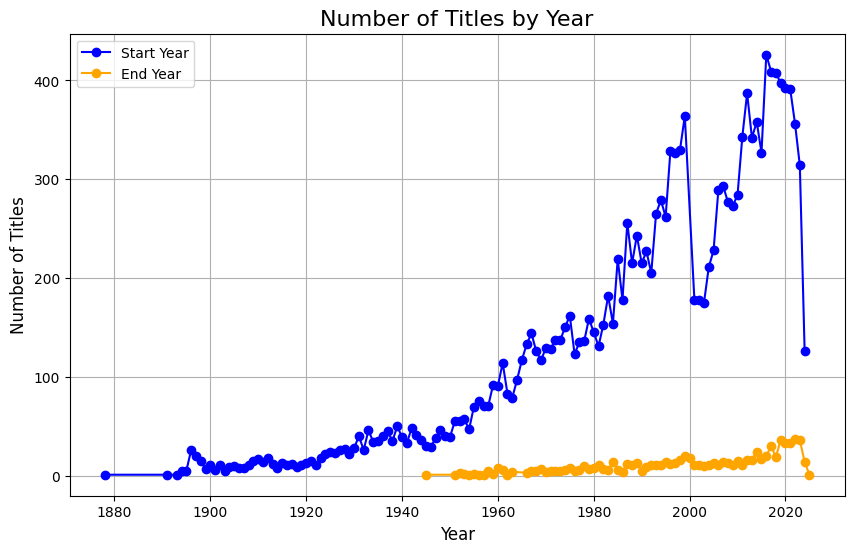
\includegraphics[width=\columnwidth]{../results/images/timeline_graph.png}
    \caption{Time series: number of titles being released and ended by year.}
    \label{fig:timeline_graph.png}
\end{figure}

In order to have a first global view of both the univariate distribution of the numeric variables singularly, and of possible interesting pairwise correlations, we build a pairplot with a KDE graph for each variable in the diagonal.
Our previous intuition about a positive correlation between \textit{startYear} and \textit{endYear} is proved by the scatterplot in Figure \ref{fig:scatterplot_endYear_startYear.png}, therefore we drop \textit{endYear}, which is more problematic due to the large number of missing values.

\begin{figure}
    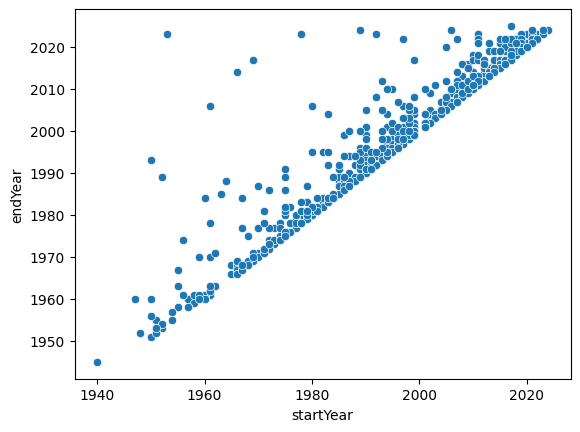
\includegraphics[width=\columnwidth]{../results/images/scatterplot_endYear_startYear.png}
    \caption{Scatterplot endYear\textasciitilde startYear.}
    \label{fig:scatterplot_endYear_startYear.png}
\end{figure}

Most numeric features (\textit{awardWins}, \textit{numVotes}, \textit{totalImages}, \textit{totalVideos}, \textit{totalCredits}, \textit{criticReviewsTotal}, \textit{awardNominationsExcludeWins}, \textit{awardsAndNominations}, \textit{numRegions}, \textit{userReviewsTotal}, \textit{numCountriesOfOrigin}, \textit{reviewsTotal}) have heavily right-skewed distributions. It makes sense that the distribution of these types of features would approximate a power law. We can address this problem using a log transformation of these features.

On the other hand, \textit{runtimeMinutes} also has a right-skewed distribution, but it really doesn't make sense for it to approximate a power law. When excluding outliers (values higher than 3rd quartile + 1.5 IQR), we can see that, for the most part, runtimes are dependent on the title type and that the distribution of the runtime for each title type approximates a bell curve (Figure \ref{fig:kde_runtimeMinutes_doppio.png}); therefore, we prefer not to log transform this variable and be mindful of the presence of outliers. Examining the titles with a longer runtime reveals that part of the outliers is due to the inconsistent strategy used for the computation of the runtime for serialized titles (series and miniseries): in some cases, the episode runtime is provided, in others, it reports the runtime for the entire series, i.e. the sum of all its episodes' runtimes (some examples are reported in Table \ref{tab:outliers_runtime}).

\begin{figure*}
    \centering
    %\includegraphics[width=\textwidth]
    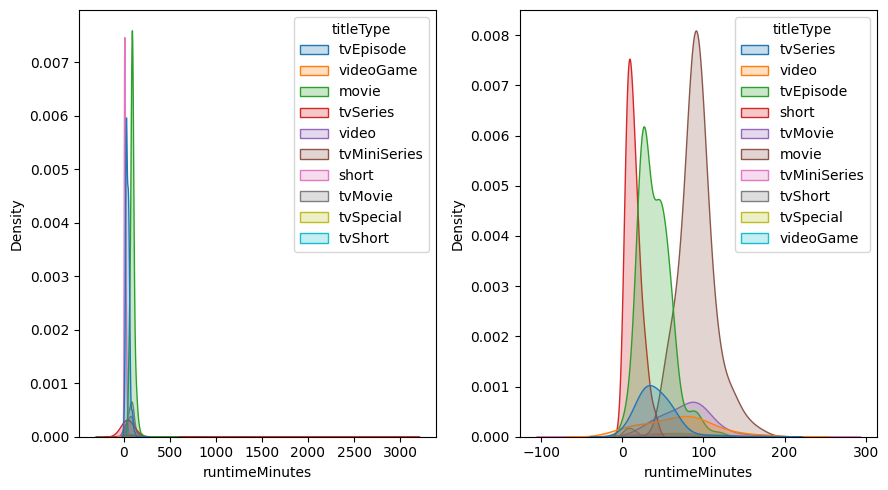
\includegraphics[width=0.6\textwidth]{../results/images/kde_runtimeMinutes_doppio.png}
    \caption{KDE for runtimeMinutes per title type, including and excluding outliers.}
    \label{fig:kde_runtimeMinutes_doppio.png}
\end{figure*}


\begin{table}[h]
    \centering
    \resizebox{\columnwidth}{!}{%
    \small
    \begin{tabular}{|p{2.7cm}|p{2.2cm}|p{1.6cm}|}
        \hline
        \textbf{originalTitle} & \textbf{runtimeMinutes} & \textbf{titleType} \\ \hline
        Alim Dayı & 3000 & tvSeries \\
        Jerry Lewis MDA Labor Day Telethon & 1290 & tvSeries \\
        Voice of the Planet & 600 & tvMiniSeries \\
        Orbius & 570 & movie \\
        Heritage: Civilization and the Jews & 540 & tvSeries \\ \hline
    \end{tabular}
    }
    \caption{Top 5 titles with the longest runtime.}
    \label{tab:outliers_runtime}
\end{table}


\subsection{Handling Missing Values}
As explained in Subsection \ref{data_semantics} and summarized in Table \ref{tab:feats_nan}, four variables in the dataset have been found to contain missing values: \textit{endYear}, \textit{runtimeMinutes}, \textit{awardWins}, \textit{genres}.

In Subsection \ref{numeric_vars_analysis}, we opted to drop \textit{endYear} because its value was missing for most records. This decision is corroborated by the fact that, on one side, it heavily correlates with \textit{startYear}, and on the other, the only records that do have an end year are of the type \textit{tvSeries} and \textit{tvMiniSeries}, and the information about the serial nature of media is already carried by the feature \textit{canHaveEpisodes}.

\textit{awardWins} has almost three thousand missing values. Given its highly unbalanced distribution, with the large majority of the records having no awards, it makes sense to fill them with the most frequent value, i.e. zero.

The stratified barplot in Figure \ref{fig:stratified_barplot_genres_titleTypes.png} shows that there is some variation in the frequency of different genres with respect to \textit{titleType}. We decided to fill the 382 missing values for \textit{genres} with the most frequent list of genres given the title type of the record, as shown in Table \ref{tab:title_types_top_nan}.

\begin{figure}
    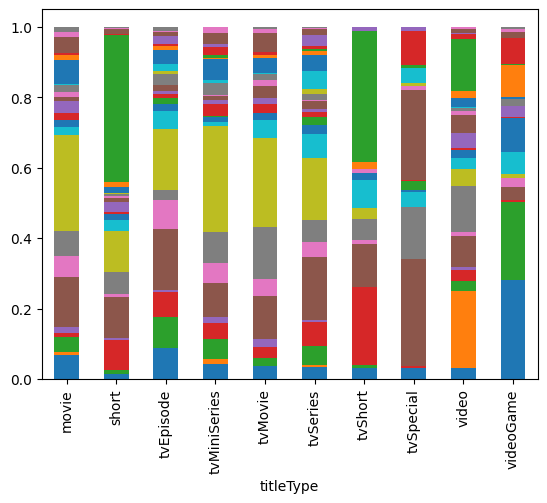
\includegraphics[width=\columnwidth]{../results/images/stratified_barplot_genres_titleTypes.png}
    \caption{Title type frequency grouped by genre.}
    \label{fig:stratified_barplot_genres_titleTypes.png}
\end{figure}

\begin{table}[h]
    \centering
    \small
    \resizebox{\columnwidth}{!}{%
    \begin{tabular}{|l|l|r|}
    \hline
    \textbf{titleType} & \textbf{top} & \textbf{\# NaN} \\ \hline
    movie & [Drama] & 230 \\
    tvSeries & [Comedy] & 53 \\
    tvMovie & [Drama] & 25 \\
    video & [Adult] & 23 \\
    tvSpecial & [Comedy] & 18 \\
    tvMiniSeries & [Drama] & 15 \\
    videoGame & [Action, Adventure, Fantasy] & 12 \\
    tvEpisode & [Comedy] & 6 \\ \hline
    \end{tabular}
    }
    \caption{Top genre for each title type with missing values for \textit{genres}.}
    \label{tab:title_types_top_nan}
\end{table}

As previously mentioned in Subsection \ref{numeric_vars_analysis}, \textit{runtimeMinutes} is dependent on the \textit{titleType} of a record (cf. Figure \ref{fig:kde_runtimeMinutes_doppio.png}): movies are generally longer than TV episodes, and shorts are typically shorter than both. Since we have some missing values for \textit{runtimeMinutes}, we can use the median value for the respective type to fill them (Table \ref{tab:median_runtime}).
\begin{table}[h]
    \centering
    \begin{tabular}{|l|c|}
    \hline
    \textbf{titleType} & \textbf{median runtime} \\ \hline
    movie & 90 \\ \hline
    short & 12 \\ \hline
    tvEpisode & 40 \\ \hline
    tvMiniSeries & 60 \\ \hline
    tvMovie & 86 \\ \hline
    tvSeries & 31 \\ \hline
    tvShort & 10 \\ \hline
    tvSpecial & 60 \\ \hline
    video & 76 \\ \hline
    videoGame & 28 \\ \hline
    \end{tabular}
    \caption{Median runtime (in minutes) by title type.}
    \label{tab:median_runtime}
\end{table}

\subsection{Pairwise correlations and eventual elimination of variables}
We observed pairwise linear correlation among numerical variables (after operating the log transformation detailed in Subsection \ref{numeric_vars_analysis}) by computing their correlation heatmap, displaying Pearson’s correlation coefficient for each pair of features (Figure \ref{fig:heatmap_first.png}).

\begin{figure*}
    \centering
    %\includegraphics[width=\textwidth]
    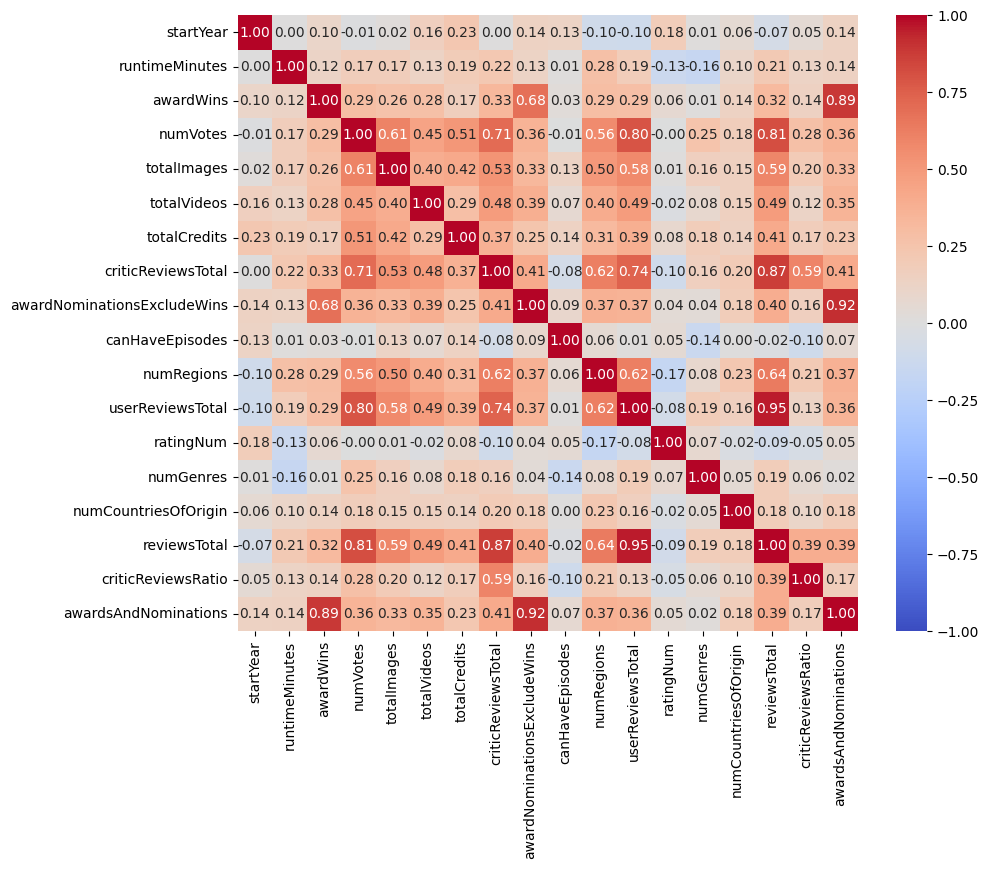
\includegraphics[width=0.7\textwidth]{../results/images/heatmap_first.png}
    \caption{Correlation heatmap before attribute removal.}
    \label{fig:heatmap_first.png}
\end{figure*}


\textit{numVotes}, \textit{userReviewsTotal}, \textit{criticReviewsTotal} and \textit{reviewsTotal} are all highly positively correlated with each other (with a correlation coefficient greater than 70). We only keep \textit{numVotes}, which has the least skewed distribution.

Since the distribution of awards and nominations is not simply skewed, but the majority of records received neither, we binarize \textit{awardsAndNominations} (Table \ref{tab:awards_nominations_bool}) and drop both \textit{awardWins} and \textit{awardNominationsExcludeWins}.

\begin{table}[h]
    \centering
    \renewcommand{\arraystretch}{1}
    \begin{tabular}{|c|c|}
        \hline
        \multicolumn{2}{|c|}{\textbf{awardsAndNominations}} \\ \hline
        False & 13692 \\ \hline
        True  & 2739 \\ \hline
    \end{tabular}
    \caption{\textit{awardsAndNominations} boolean values counts.}
    \label{tab:awards_nominations_bool}
\end{table}

Again, the majority of records do not have videos: we drop \textit{totalVideos} and substitute it with a boolean feature, \textit{hasVideos} (Table \ref{tab:hasVideos_bool}).
\begin{table}[h]
    \centering
    \renewcommand{\arraystretch}{1}
    \begin{tabular}{|c|c|}
        \hline
        \multicolumn{2}{|c|}{\textbf{hasVideos}} \\ \hline
        False & 14821 \\ \hline
        True  & 1610 \\ \hline
    \end{tabular}
    \caption{\textit{hasVideos} boolean values counts.}
    \label{tab:hasVideos_bool}
\end{table}

Similarly, most records only have one country of origin, thus we substitute \textit{numCountriesOfOrigin} with the boolean \textit{moreCountriesOfOrigin} (Table \ref{tab:moreCountriesOfOrigins_bool}).
\begin{table}[h]
    \centering
    \renewcommand{\arraystretch}{1}
    \begin{tabular}{|c|c|}
        \hline
        \multicolumn{2}{|c|}{\textbf{moreCountriesOfOrigin}} \\ \hline
        False & 15285 \\ \hline
        True  & 1146 \\ \hline
    \end{tabular}
    \caption{\textit{moreCountriesOfOrigin} boolean values counts.}
    \label{tab:moreCountriesOfOrigins_bool}
\end{table}

The overall number of features was reduced from 23 to 18; they are listed in Tables \ref{tab:dataset_numeric} and \ref{tab:dataset_categorical}. Among the remaining numeric features, we observe in the heatmap in Figure \ref{fig:heatmap_second.png} that \textit{numVotes} positively correlates to \textit{totalImages} (0.61, moderate to high correlation), to \textit{numRegions} (0.56, moderate correlation), and to \textit{totalCredits} (0.51, low-moderate correlation).

\begin{figure*}
    \centering
    %\includegraphics[width=\textwidth]
    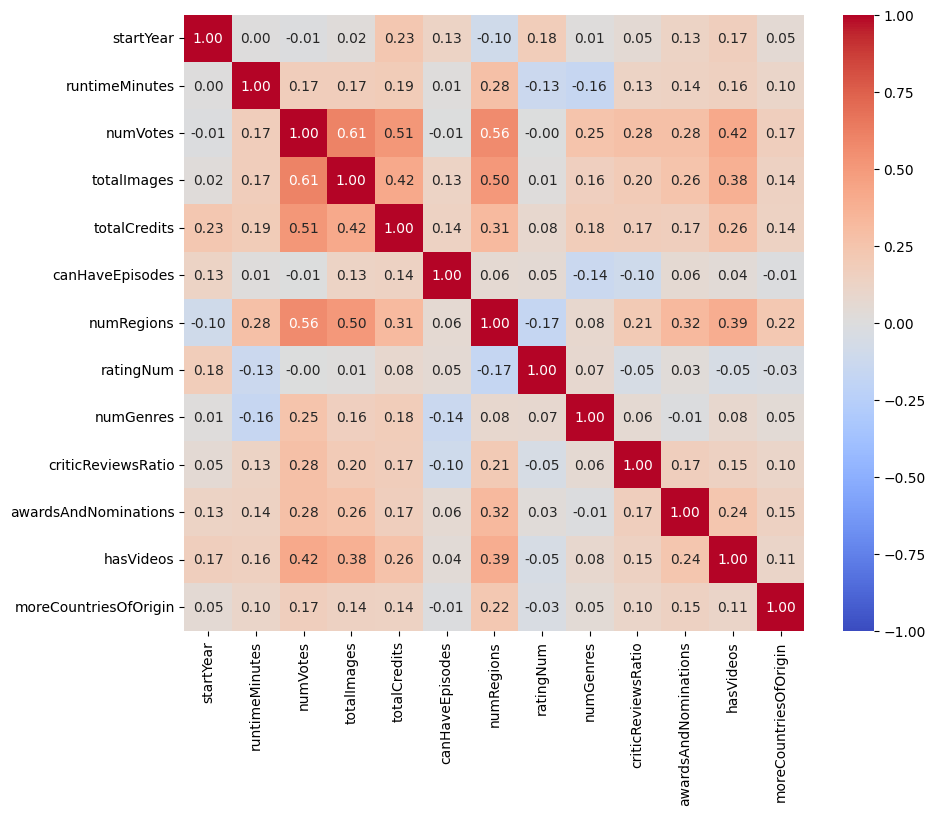
\includegraphics[width=0.7\textwidth]{../results/images/heatmap_second.png}
    \caption{Correlation heatmap after attribute removal.}
    \label{fig:heatmap_second.png}
\end{figure*}

\begin{table*}[h]
    \centering
    \renewcommand{\arraystretch}{1.2}
    \scriptsize
    \begin{tabular}{|p{3cm}|p{6cm}|p{3cm}|}
    \hline
    \textbf{Feature} & \textbf{Description} & \textbf{Type} \\ \hline
    runtimeMinutes & Primary runtime of the title, in minutes. & Continuous. Ratio-scaled. \\ \hline
    startYear & Represents the release year of a title. In the case of TV Series, it is the series’ start year. & Discrete. Interval. \\ \hline
    numVotes & Number of votes the title has received. & Discrete. Ratio-scaled. Log-transformed. \\ \hline
    numRegions & The regions number for this version of the title. & Discrete. Ratio-scaled. Log-transformed. \\ \hline
    totalImages & Total number of images for the title within the IMDb title page. & Discrete. Ratio-scaled. Log-transformed. \\ \hline
    totalCredits & Total number of credits for the title. & Discrete. Ratio-scaled. Log-transformed. \\ \hline
    criticReviewsRatio & The proportion of reviews from critics on the total number of reviews of a record. For unreviewed records, it is set to 0. & Continuous. Ratio-scaled. \\ \hline
    awardsAndNominations & Total number of awards and nominations. & Discrete. Ratio-scaled. Log-transformed. \\ \hline
    numGenres & The number of genres listed for the variable \textit{genres}. & Discrete. Ratio-scaled. \\ \hline
    \end{tabular}
    \caption{Final numeric attributes.}
    \label{tab:dataset_numeric}
\end{table*}


\begin{table*}[h]
    \centering
    \renewcommand{\arraystretch}{1.2}
    \scriptsize
    \begin{tabular}{|p{3cm}|p{6cm}|p{3cm}|}
    \hline
    \textbf{Feature} & \textbf{Description} & \textbf{Type} \\ \hline
    originalTitle & Original title, in the original language. & Categorical; mostly unique classes (i.e. names). \\ \hline
    titleType & The type/format of the title (e.g. movie, short, tvseries, tvepisode, video, etc.). & Categorical, 10 classes. \\ \hline
    countryOfOrigin & The country where the title was primarily produced. & Categorical, 153 classes. Some titles can belong to more than 1 class. \\ \hline
    genres & The genre(s) associated with the title (e.g., drama, comedy, action). & Categorical, 29 classes. Some titles can belong to more than 1 class. \\ \hline
    rating & IMDB title rating class. & Ordinal, 10 values. \\ \hline
    ratingNum & Mapping of \textit{rating} to the integers [1,10]. & Ordinal, 10 values. \\ \hline
    canHaveEpisodes & Whether or not the title can have episodes. & Asymmetric binary. \\ \hline
    hasVideos & Whether or not the title IMDb title page has at least one video. & Asymmetric binary. \\ \hline
    moreCountriesOfOrigin & Whether or not the title was produced in more than one country. & Binary. \\ \hline
    \end{tabular}
    \caption{Final categorical, ordinal, and binary attributes.}
    \label{tab:dataset_categorical}
\end{table*}
